\documentclass{szzclass}

\usepackage{amsmath}
\usepackage{graphics}
\usepackage[export]{adjustbox}[2011/08/13]
% \usepackage[czech]{babel}
% \usepackage[margin=3cm]{geometry}
% \usepackage{wrapfig}

% % spacing
% \usepackage{titlesec}
% % \titlespacing*{\section}{0pt}{1ex}{0.5ex}
% \titlespacing*{\subsection}{0pt}{1ex}{0ex}

\topic{Asymetrické kryptosystémy (šifra RSA, Diffie-Hellman, RSA digitální podpis), hešovací funkce (SHA-2, HMAC).}
\renewcommand*\contentsname{Obsah}
\author{Jakub Rathouský}
\code{BI-SPOL-06}
\subject{BEZ}

\begin{document}
% \maketitle
\tableofcontents
\newpage

\section{Asymetrické kryptosytémy}
\begin{itemize}
    \item pro šifrování a dešifrování se používá rozdílného klíče
    \item používají se soukromé klíče (SK) a veřejné klíče (VK)
    \item šifruje se pomocí VK a dešifruje pomocí SK
    \item SK se nedá z VK v rozumném čase zjistit
\end{itemize}
\section{RSA}
\begin{itemize}
    \item zabezpečení utajené komunikace
    \item každá dvojice používá šifrovací klíč
    \begin{itemize}
        \item pokud je klíč známý => dešifrovací klíč vygenerovatelný pomocí malého počtu operací
    \end{itemize}
    \item šifrovací systém VK je řešením problému s přidělováním klíče
    \begin{itemize}
        \item skládá se z veřejného klíče (VK) a tajného klíče (SK)
        \item vypočítat dešifrovací transformaci ze šifrovací je problému
        \item pomocí VK zřízena komunikace s několika subjekty
        \item každý subjekt má VK a SK pro daný šifrovací systém
        \item subjekt si ponechá určité utajené soukromé informace vnesené do konstrukce šifrovací transformace pomocí SK
    \end{itemize}
    \item seznam klíčů $VK_1, VK_2,\dots,VK_n$ je veřejný
    \item subjekt 1 vyšle zprávu $m$ subjektu 2:
    \begin{itemize}
        \item zpráva = blok (obvykle 1) určité délky; bloku OT $m$ odpovídá blok ŠT, písmena -> numerické ekvivalenty
        \item subjekt 2 s použitím dešifrovací transformace dešifruje blok ŠT
    \end{itemize}
    \item dešifrovací transformaci nelze najít v rozumném čase bez znalosti klíče
\end{itemize}
Definice:
\begin{itemize}
    \item $p$ a $q$ jsou prvočísla
    \item $n = p*q$, $\Phi(n) = (p - 1)(q - 1)$
    \item zvolí se $e$, $1 < e < n$, gdc($e$, $\Phi(n)$) = 1 a spočte se $d = |e^{-1}|_{\Phi(n)}$
    \item VK = (n, e) - ten se zveřejní
    \item SK = (d, e) - soukromý
\end{itemize}
\subsection{Princip systému}
\begin{itemize}
    \item šifrovací systém VK a je založený na modulárním umocňování
    \item dvojice ($e$, $n$) je VK; $e$ - exponent, $n$ - modul
    \item n = součin dvou privočísel $p$ a $q$, tj. $n = p*q$ a gcd($e$,$\Phi(n)$) = 1
    \item zašifrování OT: písmena = numerické ekvivalenty, vytváří se bloky s největší možnou velikostí (se sudým počtem číslic)
    \item pro zašifrování zprávy $m$ na ŠT $c$ se použije vztah:
    \begin{itemize}
        \item $E(m) = c = |m^e|_n, 0 < c < n$
    \end{itemize}
    \item pro dešifrování se použije inverze $d$ čísla $e$ modulo $\Phi(n)$ (existuje protože gcd($e$, $\Phi(n)$) = 1))
    \item pro dešifrování bloku $c$ platí:
    \begin{itemize}
        \item D($c$) = $|c^d|_n = |m^{ed}|_n = |m^{k*\Phi(n)+1}|_n = |(m^{\Phi(n)})^k*m|_n = |m|_n$
        \item kde $e*d = k*\Phi(n) + 1$ pro nějaké celé číslo $k (|ed|_{\Phi(n)} = 1)$ a z Eulerovy věty platí $|p^{\Phi(n)}|_n = 1$, kde gcd($p$, $n$) = 1
    \end{itemize}
    \item dvojice (d, n) je dešifrovací klíč - tajná část klíče
\end{itemize}
\begin{figure}[h!]
    \centering
    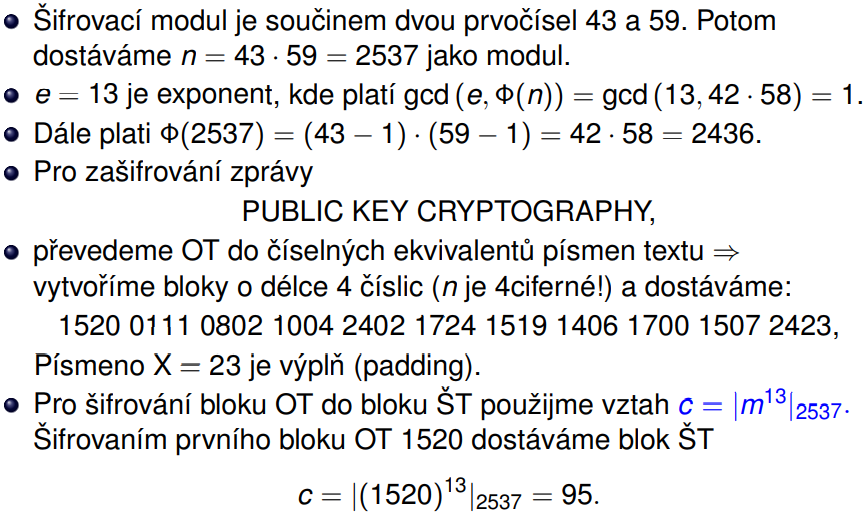
\includegraphics[width=0.8\textwidth]{topics/bi-spol-06/image/rsaEncrypt.png}
    \caption{Zašifrování pomocí RSA}
\end{figure}
\begin{figure}[h!]
    \centering
    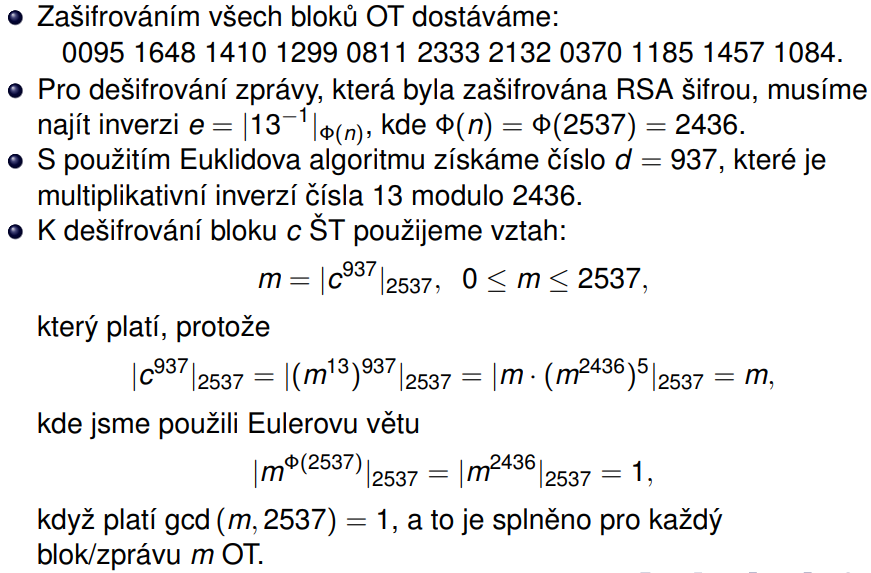
\includegraphics[width=0.8\textwidth]{topics/bi-spol-06/image/rsaDecrypt.png}
    \caption{Dešifrování RSA}
\end{figure}
\subsection{Bezpečnost}
\begin{itemize}
    \item modulární umocnění potřebné k šifrování zprávy s použitím RSA může být provedeno při VK a $m$ o velikosti $~200$ dekadických číslic za několik sekund
    \item se znalostí $p$ a $q$ a s použítím Euklidova algoritmu lze najít dešifrovací klíč $d$
    \item bez znalosti prvočísel $p$ a $q$ není lehké nalézt dešifrovací klíč, najít je pomocí $\Phi(n)$ je podobně složité jako faktorizace celého čísla $n$
\end{itemize}
\subsubsection{Problém faktorizace}
\begin{itemize}
    \item jedná se o převedení čísla na součin jeho faktorů (rozklad na prvočísla)
    \item pokud $p$ a $q$ jsou 100číslicová prvočísla, tak pak $n$ je 200číslicové
    \item nejrychlejší známý algoritmus potřebuje pro faktorizaci $~10^6$ roků k faktorizci takového čísla
    \item naopak, pokud je známo d, ale nezná se $\Phi(n)$, je možné lehce faktorizovat n, protože se ví, že $e*d - 1$ je násobkem $\Phi(n)$
    \item čím větší modulo, tím je výpočet náročnější
    \item ochrana proti speciálním rychlým technikám:
    \begin{itemize}
        \item obě hodnoty $p-1$ a $q-1$ by měly mít velký prvočíselný faktor
        \item gcd($p-1$, $q-1$) by mělo být malé a $p$ a $q$ by měly mít rozdílnou desítkovou reprezentaci v délce několika málo číslic
    \end{itemize}
\end{itemize}

\section{RSA digitální podpis}
\begin{itemize}
    \item RSA lze použít pro vyslání podepsané zprávy
    \item při použití podpisu se příjemce může ujistit, že:
    \begin{itemize}
        \item zpráva přišla od oprávněného odesílatele
        \item a je tomu tak na základě nestranného a objektivního testu
    \end{itemize}
    \item takové ověření je potřeba pro elektronickou počtu, elektronické bankovnictví, elektronický obchod\dots
\end{itemize}
\subsection{Princip}
\begin{itemize}
    \item subject 1 vysílá podepsanou zprávu $m$
    \item subjekt 1 spočítá pro zprávu $m$ OT
    \begin{itemize}
        \item $S = D_{SK_1}(m) = |m^{d_1}|_{n_1}$
        \item kde $SK_1$ = ($d_1, n_1$) je tajný klíč pro subjekt 1
    \end{itemize}
    \item když $n_2 > n_1$, kde $VK_1$ = ($e_2$,$n_2$) je veřejný šifrovací klíč pro subjekt 2, subjekt 1 zašifruje S pomocí vztahu
    \begin{itemize}
        \item $c = E_{VK_2}(S) = |S^{e_2}|_{n_2}$
        \item $0 < c < n_2$
    \end{itemize}
    \item když $n_2 < n$ subjekt 1 rozdělí S do bloků o velikosti menší než $n_2$ a zašifruje každý blok s použitím šifrovací transformace $E_{VK_2}$
    \item pro dešifrování subjekt 2 nejdříve použije soukromou dešifrovací transformaci $D_{SK_2}$ k získání S, protože
    \begin{itemize}
        \item $D_{SK_2}(c) = D_{SK_2}(E_{VK_2}(S)) = S$
    \end{itemize}
    \item k nalezení OT $m$ subjekt dále použije veřejnou šifrovací transoformaci $E_{VK_1}$, protože
    \begin{itemize}
        \item $E_{VK_1}(S) = E_{VK_1}(D_{SK_1}(m)) = m$
    \end{itemize}
    \item kombinace OT $m$ a podepsané verze S přesvědčí subjekt 2, že zpráva byla vyslána subjektem 1
    \item také subjekt 1 nemůže odepřít, že on vyslal danou zprávu, žádný jiný subjekt než 1 nemůže generovat podepsanou zprávu S z originálního textu zprávy $m$
\end{itemize}
\begin{figure}[h!]
    \centering
    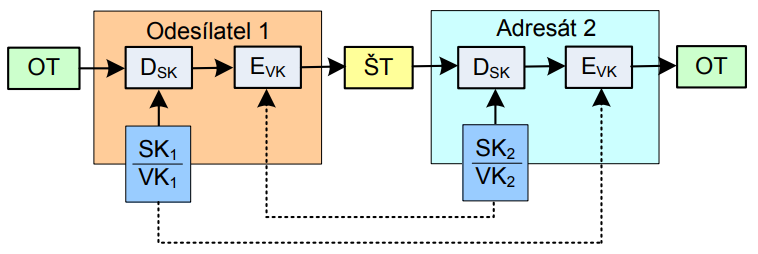
\includegraphics[width=0.8\textwidth]{topics/bi-spol-06/image/digitalSubscription.png}
    \caption{Šifrování digitálního podpisu}
\end{figure}
\section{Diffie-Hellman}
Vhodná šifra pro zřízení společného kníče pro dva a více subjektů. První účastník zvolí modulo $m$ a číslo $a$.
Každý objekt si zvolí svůj privátní klíč $k$.
Musí platit:
\begin{itemize}
    \item gcd(m, a) = 1
    \item gcd($k_i$, m-1) = 1
\end{itemize}
\subsection{Princip}
\begin{itemize}
    \item volba veřejných prvků účastníkem A: $m$ prvočíslo a $a$ celé číslo $\rightarrow 0 < a < m$
    \item generování parametrů klíče účastníkem A: volba čísla $k_1 < m$ a výpočet $y_1 = |a^{k_1}|_m$
    \item účastník A odešle účastníkovi V čísla $a, m$ a $y_1$
    \item generování parametrů klíče účastníkem B: volba čísla $k_2 < m$ a výpočet $y_2 = |a^{k_2}|_m$
    \item účastník B odešle účasníkovi A číslo $y_2$
    \item generování společného klíče Ačkem: $K = |Y^{k_1}_2|_m$
    \item generování společného klíče Bčkem: $K = |Y^{k_2}_1|_m$
    \item veřejnými prvky jsou čísla $m$ a $a$
    \item neautorizovaný subjekt nemůže najít společný klíč $K$ v rozumném čase, protože je nucen hledat logaritmus modulo $m$
\end{itemize}
\begin{figure}[h!]
    \centering
    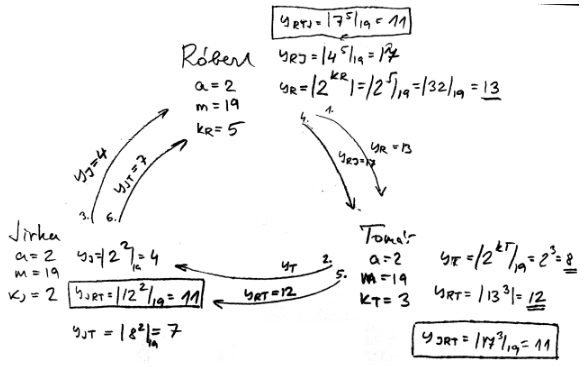
\includegraphics[width=0.8\textwidth]{topics/bi-spol-06/image/DH.png}
    \caption{Diffie-Hellman pro 3 osoby}
\end{figure}
\subsection{Bezpečnost}
\begin{itemize}
    \item délka klíče je přímo uměrná kvalitě šifry
    \item když je $m$ prvočíslo a $m-1$ je součin malých prvočísel $\rightarrow$ je možné pomocí speciální metody nalézt logaritmus modulo $m$ méně operacemi než $O(log^2_2m)$
\end{itemize}
\subsection{Problém diskrétního logaritmu}
\begin{itemize}
    \item $C = t^k (mod p)$
    \item pokud se zná t, k a p $\Rightarrow$ C se spočítá snadno
    \item inverzní operace je ale náročná - tzn. spočítat k ke znalosti t, p a C
    \item $k = |log_t(C)|_p$, k = diskrétní logaritmus
\end{itemize}
\section{Hešovací funkce}
Silný nástroj moderní kryptografie. Jedna z klíčových kryptologických myšlenek. Základní pojmy: \textit{jednosměrnost} a \textit{bezkoliznost}.
\newline
\begin{itemize}
    \item původní význam hešovací funkce byla funkce, která libovolně velkému vstupu přiřadila krátký hash kód o pevně definované délce
    \item v součastnosti se pojem hash funkce používá v kryptografii pro krypto-hash funkce, která má oproti původní definici ještě navíc vlastnosti \textit{jednosměrnost} a \textit{bezkoliznost}
\end{itemize}
Vezme se přirozené číslo $d$ a množina $X$ všech binárnách řetězců délky 0 až $d$. Funkce $f: X -> \{0, 1\}^n$ se nazve hešovací,
pokud je jednosměrná \texttt{1. typu} a \texttt{bezkolizní}. Každému binárnímu řetězci z množiny X přiřadí binární hash-kód délky $n$ bitů.
\subsection{Vstup a výstup}
\begin{itemize}
    \item hash funkce h zpracovává prakticky neomezeně dlouhá vstupní data M na krátký výstupní hash kód h(M) pevné a předem stanovené délky
\end{itemize}
Z hlediska bezpečnosti se požaduje, aby se hešovací funkce chovala jako náhodné orákulum:
\begin{itemize}
    \item orákulum = libovolný nástroj, který na základě vstupu odpoví nějakým výstupem. Na ten samý vstup, musí odpovědět stejně
    \item náhodné orákulum - orákulum, které na nový vstup odpoví náhodným výběrem výstupu z množiny výstupů
\end{itemize}
\subsection{Jednosměrnost}
Funkce $f: X \rightarrow Y$, pro něž je snadné z jakékoli hodnoty $x \in X$ vypočítat $y = f(x)$, ale pro nějaký náhodně vybraný obraz $y \in f(X)$ nelze
najít její vzor $x \in X$ tak, aby $y = f(x).$
\newline
Jednosměrné funkce se dělí na:
\begin{itemize}
    \item jednosměrné, pro které je výpočetně nemožné, ale teoretický existující, najít vzor z obrazu
    \item jednosměrné funkce s padacími vrátky, u kterých lze najít vzor z obrazu, ale jen za předpokladu znalosti "padacích vrátek" - klíče
\end{itemize}
\begin{figure}[h!]
    \centering
    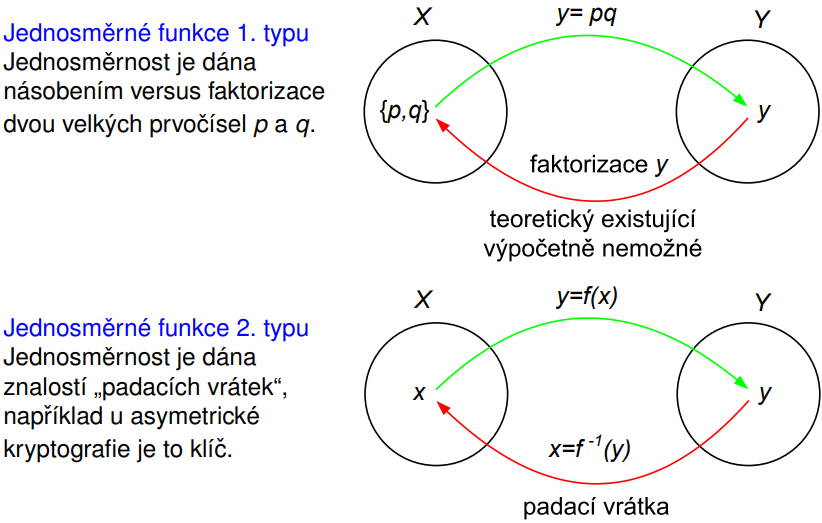
\includegraphics[width=0.6\textwidth]{topics/bi-spol-06/image/oneWayHashFunction.png}
    \caption{Jednosměrné funkce}
\end{figure}
\subsection{Bezkoliznost}
\subsubsection{Bezkoliznost 1. řádu}
Je odolnost proti kolizi a požaduje, aby bylo výpočetně nezvládnutelné nalezení libovolných dvou různých zpráv tak, že budou mít stejnou hash.
Pokud k tomu dojde, tak se nalezla kolize. (lidsky: pro dvě lib. se nesmí zjistit, že se zahashují stejně)
\begin{itemize}
    \item bezkoliznost se zásadně využívá k digitálním podpisům
    \item nepodepisuje se přímo zpráva, ale pouze její hash
    \item bezkoliznost zaručuje, že není možné nalézt dva dokumenty se stejnou hash
\end{itemize}
\subsubsection{Bezkoliznost 2. řádu}
Hashovací funkce $h$ je odolná proti nalezení 2. vzoru, jestliže pro daný náhodný vzor x je výpočetně nezvládnutelné nalézt 2. jiný vzor tak, že se
zahashují stejně. (lidsky: máme vzor a nesmíme k tomu najít druhý, aby se zahashovaly stejně)
\subsection{Konstrukce moderních hash funkcí}
Moderní hash funkcí, může být velmi dlouhá. Zpráva se proto zpracovává po částech. Nutnost hashování po blocích a zarovnávat vstupní zprávy na celistvý počet bloků.
Zarovnání musí být bezkolizní a umožňovat jednoznačné odejmutí.
\subsubsection{Zarovnání}
Zarovnání musí být jednoznačné, aby nevznikly jednoduché kolize. Doplněním například 0 bitem by způsobilo zmatek, který poslední nultý bit je platný.
U nových hash funkcí se doplní bit 1 a pak zbytek 0. Tím se rozezná, kde je konec zprávy.
\subsubsection{Damgard-Merklovo zesílení}
Jedná se o doplnění o délku původní zprávy. Zpráva je doplněna bitem 1 a pak bity 0 tak, aby na konci zbylo 64 bitů volných. Do nich je vyplněna hodnota
 bitů původní zprávy. Začlenění informace o délce původní zprávy eliminuje případné útoky. Současné hash funkce používají DM princip iterativně s využitím kompresní funkce.

Kompresní metoda zpracuje aktuální blok zprávy a výsledek je určitá hodnota, která nutně tvoří vstup do další iterace. Ta funkce má dva vstupy, předchozí krok a další blok.
Prvotní zavolání obsahuje první blok a definovanou konstantu, která se říká \textit{inicializační hodnota}.

\subsection{SHA-2}
Pod SHA-2 patří SHA-(224/256/384/512).

Založen na Damgard-Merklově konstrukci:
\begin{itemize}
    \item je to iterativní konstrukce
    \item f zpracovává aktuální blok zprávy $M_i$ a výsledek je kontext $H_i$
    \item $H_i$ nutně tvoří vstup do f v dalším kroku
    \item f má tedy vstupy $H_{i-1}$ a $M_i$
\end{itemize}

\begin{figure}[h!]
    \centering
    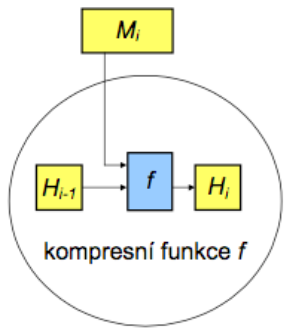
\includegraphics[width=0.6\textwidth]{topics/bi-spol-06/image/sha2.png}
    \caption{SHA2 kompresní funkce}
\end{figure}

SHA = Secure Hash Algorithm
\begin{itemize}
    \item nástupce SHA-1
    \item nejvýznamější rozdíly jsou v délce hashovacího kódu, který určuje odolnost hashového kodu vůči
     nalezení kolizí 1. a 2. řádu
\end{itemize}

\begin{figure}[h!]
    \centering
    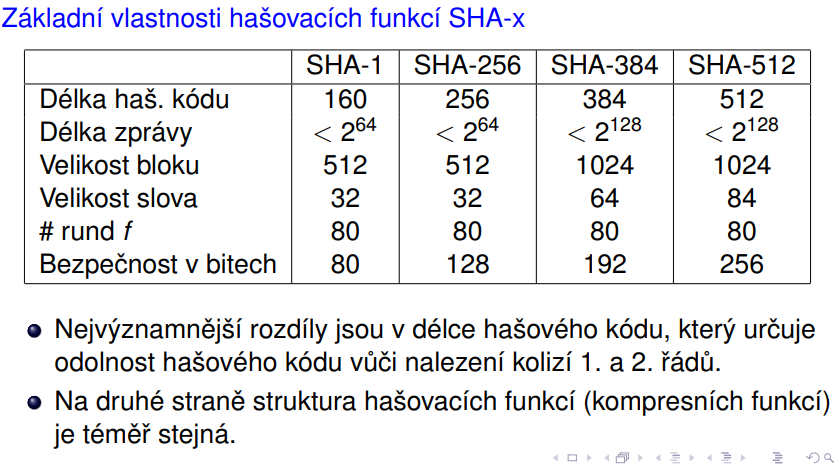
\includegraphics[width=0.6\textwidth]{topics/bi-spol-06/image/shaCompare.png}
    \caption{Porovnání SHA funkcí}
\end{figure}

\subsection{HMAC}
Klíčované hashované autentizační kódy zpráv HMAC zpracovávají hashováním nejen zprávu M, ale spolu s ní i nějaký tajný klíč K.
Jsou proto podobné autentizačnímu kódu zprávy MAC, ale místo blokové šifry se použije hashovací.

Používají se k nepadělatelnému zabezpečení zpráv a autentizaci (prokázáním znalosti tajného klíče). HMAC je obecná konstrukce, která využívá obecnou hashovací funkci.
Podle konkrétní hashovací funkce, která se konkrétně používá, se označuje výsledná funkce (HMAC-SHA-1(M, K) používá sha-1, kde M je zpráva a K je tajný klíč).
\subsubsection{Algoritmus}
Definuje se konstantní řetězen \textit{ipad} jako řetězec b/8 bajtů s hodnotou 0x36 a \textit{opad} jako řetězec b/8 bajtů s hodnotou 0x5C.
Klíč $K$ se doplní bity 0 vlevo od MSB bitu klíče do délky b-bitu a označí se $K^+$. Definuje se hodnota $HMAC_k(M)$ jako:
\begin{center}
$HMAC_k(M) = H((K^+ \oplus opad)||((K^+ \oplus ipad)||M))$
\end{center}
\subsubsection{Nepadělatelnost}
Pokud je kod připojen za zprávu M, detekuje neúmyslnou chybu při jejím přenosu. Zabraňuje útočníkovi změnit zprávu a současně změnit HMAC, protože
bez znalosti klíče nelze nový HMAC vypočítat. Správný HMAC je autentizací původu dat, odesílatel musel znát tajný klíč.
\subsubsection{Průkaz znalosti}
HMAC může být použit jako průkaz znalosti tajného sdíleného klíče při autentizaci entit. Dotazovatel odešlne náhodou výzvu, které se říká \textit{challenge}
a od provozovatele dostane odpověď \textit{response}. Prokazovatel zná tajný klíč. Útočník z hodnoty response klíč nemůže odvodit.
\end{document}
